% AAS Research Notes submission — compile with AASTeX v6.3.1+
% Word limit 1000 (body), one figure. Fill [BRACKETED] items before submission.
\documentclass[RNAAS]{aastex631}

\begin{document}

\title{Dynamical Stability Audits Expose Three Classes of Parameter Artifacts in Exoplanet Catalogs}

\author{Shaurya Ranjan}
\affiliation{[AFFILIATION / Independent Researcher, City, Country]}
\email{shauryaranjan911@gmail.com}

\section*{}

Aggregated exoplanet catalogs --- above all the NASA Exoplanet Archive ---
are the de facto input for population studies, dynamical analyses, and
target selection. During a homogeneous $N$-body stability survey of
multi-planet radial-velocity systems, we found that requiring a system's
own long-term survival is a sharp, inexpensive audit of its published
parameters: configurations drawn directly from the catalog sometimes
self-destruct within $10^3$--$10^4$ orbits, impossible for systems
observed to be Gyr old. Chasing every such contradiction to its root
exposed three recurring artifact classes. None is hypothetical --- each
broke a real analysis before being diagnosed.

\textbf{Class 1: eccentricity point estimates that are dynamically fatal
noise.} Compact low-mass systems are typically fit with small, poorly
constrained eccentricities whose posteriors are consistent with zero; the
catalog nonetheless records nonzero point values. Barnard's star is the
extreme case: its four sub-Earth planets (periods 2.3--6.7~d) carry
catalog eccentricities $e = 0.03$--$0.08$ with $1\sigma$ uncertainties of
the same size (e.g.\ $e = 0.040 \pm 0.040$). Integrated as written, the
system destroys itself through close encounters within 1{,}400--4{,}300~yr
in every realization; the same entry forced circular survives $10^6$
inner orbits in every realization (Figure~\ref{fig:barnard}). Neither
extreme is correct: drawing eccentricities from their published
uncertainties (truncated at zero) yields intermediate survival and
propagates the ignorance honestly. For dynamically packed systems,
catalog eccentricity point values must be treated as draws from a
distribution, never as facts.

\textbf{Class 2: composite tables mix parameters from incompatible fits.}
The Archive's \texttt{pscomppars} table assembles each parameter from the
best available reference per column, so one system's rows can combine
periods from one paper with eccentricities, periastron angles, and
periastron times from others. For resonant or near-resonant systems the
damage is acute: phases assembled across references imply timing
relationships no fit ever measured. In our survey, phases derived from
composite periastron times falsely collapsed the stable systems 47~UMa
and HD~141399 to near-total instability at their minimum masses.
Phase-sensitive dynamics requires self-consistent parameter sets from a
single reference (the \texttt{ps} table filtered to one
\texttt{pl\_refname}); composite rows are safe only with phases
discarded and parameters sampled within uncertainties.

\textbf{Class 3: fit epochs stored as times of periastron.} For some
references \texttt{pl\_orbtper} contains the \emph{epoch of the fit}
rather than periastron passage times. GJ~876 \citep{Rivera2010} is
reported with \texttt{pl\_orbtper} $= 2450602.093$ for all four planets
--- the fit epoch --- which, read literally, puts every planet at
periastron simultaneously. Phases derived from these values initialize
the 2:1 Laplace resonance far from its libration center, and the
reconstructed system --- stable in every published analysis --- is
destroyed within 5{,}000~yr even under an exact (IAS15) integration. The
correct mean anomalies ($355\arcdeg$, $294.59\arcdeg$, $325.7\arcdeg$,
$335\arcdeg$; \citealt{Rivera2010}, Table~3) restore libration. Identical
periastron times across a multi-planet system are a reliable signature of
this artifact.

\textbf{Recommendations.} (1) Treat catalog eccentricities of compact
systems as distributions bounded below by zero and marginalize stability
conclusions over them. (2) Never derive orbital phases from composite
tables. (3) Reject periastron times identical across planets. (4)
Archives could flag columns whose values are epochs rather than
measurements, and offer a dynamically self-consistent single-reference
view. Each check costs seconds; the failures they prevent masquerade
convincingly as science.

Integrations used \textsc{rebound}/WHFast \citep{ReinLiu2012,
ReinTamayo2015} with instability defined by Hill-sphere overlap or
escape. Code, per-run records, and the parent survey are available at
[REPOSITORY / Zenodo DOI]. [AI-ASSISTANCE DISCLOSURE PER JOURNAL POLICY.]

\begin{figure}[ht!]
\centering
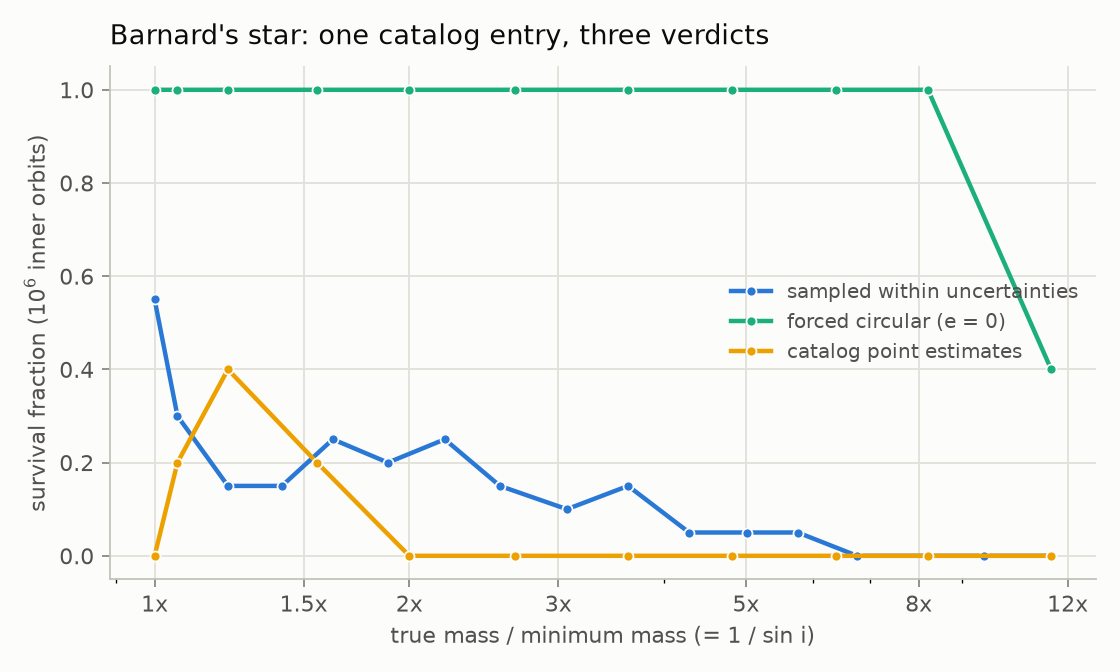
\includegraphics[width=0.85\textwidth]{note_fig1_barnard.png}
\caption{Survival fraction of Barnard's star realizations versus the
swept mass factor $1/\sin i$, integrated for $10^6$ inner-planet orbits
under three treatments of the same catalog entry: eccentricities drawn
within published uncertainties (blue), forced circular (green), and
catalog point estimates (yellow). Point estimates destroy the system even
at minimum masses; circular orbits survive nearly everywhere; sampling
propagates the uncertainty honestly.}
\label{fig:barnard}
\end{figure}

\begin{thebibliography}{}
\bibitem[Gladman(1993)]{Gladman1993} Gladman, B. 1993, Icarus, 106, 247
\bibitem[Rein \& Liu(2012)]{ReinLiu2012} Rein, H., \& Liu, S.-F. 2012, A\&A, 537, A128
\bibitem[Rein \& Tamayo(2015)]{ReinTamayo2015} Rein, H., \& Tamayo, D. 2015, MNRAS, 452, 376
\bibitem[Rivera et al.(2010)]{Rivera2010} Rivera, E.~J., Laughlin, G., Butler, R.~P., et al. 2010, ApJ, 719, 890
\end{thebibliography}

\end{document}
